\documentclass[8pt,aspectratio=169]{beamer}
\usetheme{Madrid}
\usepackage{graphicx}
\usepackage{booktabs}
\usepackage{adjustbox}
\usepackage{multicol}
\usepackage{amsmath}
\usepackage{listings}
\usepackage{xcolor}

% Color definitions
\definecolor{mlblue}{RGB}{0,102,204}
\definecolor{mlpurple}{RGB}{51,51,178}
\definecolor{mllavender}{RGB}{173,173,224}
\definecolor{mllavender2}{RGB}{193,193,232}
\definecolor{mllavender3}{RGB}{204,204,235}
\definecolor{mllavender4}{RGB}{214,214,239}
\definecolor{mlorange}{RGB}{255, 127, 14}
\definecolor{mlgreen}{RGB}{44, 160, 44}
\definecolor{mlred}{RGB}{214, 39, 40}
\definecolor{mlgray}{RGB}{127, 127, 127}

% Additional colors for template compatibility
\definecolor{lightgray}{RGB}{240, 240, 240}
\definecolor{midgray}{RGB}{180, 180, 180}

% Code listing colors
\definecolor{codegreen}{rgb}{0,0.6,0}
\definecolor{codegray}{rgb}{0.5,0.5,0.5}
\definecolor{codepurple}{rgb}{0.58,0,0.82}
\definecolor{backcolour}{rgb}{0.95,0.95,0.95}

% Apply custom colors to Madrid theme
\setbeamercolor{palette primary}{bg=mllavender3,fg=mlpurple}
\setbeamercolor{palette secondary}{bg=mllavender2,fg=mlpurple}
\setbeamercolor{palette tertiary}{bg=mllavender,fg=white}
\setbeamercolor{palette quaternary}{bg=mlpurple,fg=white}

\setbeamercolor{structure}{fg=mlpurple}
\setbeamercolor{section in toc}{fg=mlpurple}
\setbeamercolor{subsection in toc}{fg=mlblue}
\setbeamercolor{title}{fg=mlpurple}
\setbeamercolor{frametitle}{fg=mlpurple,bg=mllavender3}
\setbeamercolor{block title}{bg=mllavender2,fg=mlpurple}
\setbeamercolor{block body}{bg=mllavender4,fg=black}
\setbeamercolor{block title alerted}{bg=mlred,fg=white}
\setbeamercolor{block body alerted}{bg=red!10,fg=black}

% Remove navigation symbols
\setbeamertemplate{navigation symbols}{}

% Clean itemize/enumerate
\setbeamertemplate{itemize items}[circle]
\setbeamertemplate{enumerate items}[default]

% Reduce margins for more content space
\setbeamersize{text margin left=5mm,text margin right=5mm}

% Code listing style
\lstdefinestyle{solidity}{
    backgroundcolor=\color{backcolour},
    commentstyle=\color{codegreen},
    keywordstyle=\color{mlpurple}\bfseries,
    numberstyle=\tiny\color{codegray},
    stringstyle=\color{codepurple},
    basicstyle=\ttfamily\tiny,
    breakatwhitespace=false,
    breaklines=true,
    captionpos=b,
    keepspaces=true,
    numbers=left,
    numbersep=3pt,
    showspaces=false,
    showstringspaces=false,
    showtabs=false,
    tabsize=2,
    frame=single,
    morekeywords={contract, function, returns, return, public, private, external, internal, view, pure, payable, modifier, event, emit, mapping, address, uint256, uint8, bool, string, bytes, require, if, else, for, while, constructor, import, pragma, solidity, is, constant, override, virtual, memory, calldata, storage}
}

\lstdefinestyle{javascript}{
    backgroundcolor=\color{backcolour},
    commentstyle=\color{codegreen},
    keywordstyle=\color{mlblue}\bfseries,
    numberstyle=\tiny\color{codegray},
    stringstyle=\color{codepurple},
    basicstyle=\ttfamily\tiny,
    breakatwhitespace=false,
    breaklines=true,
    captionpos=b,
    keepspaces=true,
    numbers=left,
    numbersep=3pt,
    showspaces=false,
    showstringspaces=false,
    showtabs=false,
    tabsize=2,
    frame=single,
    morekeywords={const, let, var, function, async, await, require, console, log, return, if, else, for, while, try, catch, throw, new, this, true, false}
}

% Command for bottom annotation (Madrid-style)
\newcommand{\bottomnote}[1]{%
\vfill
\vspace{-2mm}
\textcolor{mllavender2}{\rule{\textwidth}{0.4pt}}
\vspace{1mm}
\footnotesize
\textbf{#1}
}

\title{Create Your Own Cryptocurrency}
\subtitle{Lesson 4 of 4: ERC-20 Token Creation}
\author{Cryptocurrency Development Course}
\institute{From Theory to Practice}
\date{\today}

\begin{document}

% ==================== TITLE SLIDE ====================
\begin{frame}[plain]
\vspace{1.5cm}
\begin{center}
{\Huge Create Your Own Cryptocurrency}\\[0.5cm]
{\Large Lesson 4 of 4: ERC-20 Token Creation}\\[1.5cm]
{\normalsize Building Fungible Tokens on Ethereum}\\[0.5cm]
{\small From Token Standards to Deployment}
\end{center}
\vfill
\begin{center}
\textcolor{mlgray}{\small Cryptocurrency Development Course}
\end{center}
\end{frame}

% ==================== PREREQUISITES ====================
\begin{frame}{Prerequisites}
\textbf{Before this lesson, you should understand:}
\begin{itemize}
\item Lessons 1-3: Blockchain, cryptography, and smart contracts
\item Basic JavaScript syntax (for deployment scripts)
\item How to use Node.js and npm
\end{itemize}

\vspace{1em}
\textbf{Software needed:}
\begin{itemize}
\item Node.js v18+ with npm
\item Hardhat (\texttt{npm install --save-dev hardhat})
\item OpenZeppelin contracts (\texttt{npm install @openzeppelin/contracts})
\item MetaMask (optional, for testnet deployment)
\end{itemize}

\vspace{1em}
\textbf{What you'll create:}\\
Your own cryptocurrency token on Ethereum!

\bottomnote{This is the final lesson -- bringing everything together to create a real token.}
\end{frame}

% ==================== OUTLINE ====================
\begin{frame}[t]{Lesson Outline}
\tableofcontents
\vfill
\footnotesize
\textbf{Duration:} 45 minutes | \textbf{Prerequisite:} Lessons 1-3 (Blockchain, Cryptography, Smart Contracts)
\end{frame}

% ==================== SECTION 1: TOKEN STANDARDS ====================
\section{Token Standards}

\begin{frame}[t]
\vfill
\centering
\begin{beamercolorbox}[sep=8pt,center]{title}
\usebeamerfont{title}\Large Section 1: Token Standards\par
\end{beamercolorbox}
\begin{center}
\textit{Understanding the building blocks of digital assets}
\end{center}
\vfill
\end{frame}

% ==================== SLIDE 3: WHAT IS A TOKEN? ====================
\begin{frame}[t]{What is a Token?}
\begin{columns}[T]
\column{0.48\textwidth}
\textbf{Tokens vs. Coins}

\textbf{Coins (Native Currency):}
\begin{itemize}
\item Have their own blockchain
\item Used for transaction fees
\item Examples: ETH, BTC, SOL
\end{itemize}

\vspace{0.5em}
\textbf{Tokens (Smart Contract Assets):}
\begin{itemize}
\item Built \textit{on top of} existing blockchains
\item Created via smart contracts
\item Examples: USDC, LINK, UNI
\end{itemize}

\column{0.48\textwidth}
\textbf{Token Use Cases}

\begin{itemize}
\item \textbf{Utility:} Access to services (API credits)
\item \textbf{Governance:} Voting rights (DAO tokens)
\item \textbf{Security:} Represent ownership shares
\item \textbf{Stablecoin:} Pegged to real assets
\item \textbf{NFT:} Unique digital collectibles
\item \textbf{Gaming:} In-game currencies
\end{itemize}

\vspace{0.5em}
\textbf{Key Insight:}\\
Tokens are programmable money with custom rules encoded in smart contracts.
\end{columns}

\bottomnote{Over 500,000 tokens exist on Ethereum alone, demonstrating the power of token standards}
\end{frame}

% ==================== SLIDE 4: WHY STANDARDS MATTER ====================
\begin{frame}[t]{Why Standards Matter}
\begin{columns}[T]
\column{0.48\textwidth}
\textbf{Without Standards}

\begin{itemize}
\item[\textcolor{mlred}{$\times$}] Every token has different functions
\item[\textcolor{mlred}{$\times$}] Wallets need custom code per token
\item[\textcolor{mlred}{$\times$}] Exchanges can't easily list tokens
\item[\textcolor{mlred}{$\times$}] DeFi protocols can't be composable
\item[\textcolor{mlred}{$\times$}] Security audits are complex
\end{itemize}

\vspace{0.3em}
\begin{block}{Real-World Analogy}
Without standards, tokens would be like \textbf{gift cards that only work at one specific store}. ERC-20 makes tokens like \textbf{standard gift cards} that work everywhere!
\end{block}

\column{0.48\textwidth}
\textbf{With Standards (ERC-20)}

\begin{itemize}
\item[\textcolor{mlgreen}{$\checkmark$}] Consistent interface for all tokens
\item[\textcolor{mlgreen}{$\checkmark$}] One wallet supports all tokens
\item[\textcolor{mlgreen}{$\checkmark$}] Easy exchange integration
\item[\textcolor{mlgreen}{$\checkmark$}] DeFi composability (``money legos'')
\item[\textcolor{mlgreen}{$\checkmark$}] Audited reference implementations
\end{itemize}

\vspace{0.5em}
\textbf{The Solution:}\\
ERC-20 defines what every fungible token \textit{must} implement.
\end{columns}

\bottomnote{ERC = Ethereum Request for Comments | ERC-20 was proposed in 2015 by Fabian Vogelsteller}
\end{frame}

% ==================== SLIDE 5: ERC-20 STANDARD ====================
\begin{frame}[t]{ERC-20: The Fungible Token Standard}
\begin{columns}[T]
\column{0.48\textwidth}
\textbf{What is ERC-20?}

A technical standard defining:
\begin{itemize}
\item Required functions every token must have
\item Events that must be emitted
\item Expected behavior for transfers
\end{itemize}

\vspace{0.5em}
\textbf{Fungibility:}
\begin{itemize}
\item Each token is identical
\item 1 token = 1 token (interchangeable)
\item Like dollar bills --- any \$1 equals any other \$1
\end{itemize}

\column{0.48\textwidth}
\textbf{The Standard Interface}

\vspace{0.3em}
\textbf{6 Required Functions:}
\begin{enumerate}
\item \texttt{totalSupply()}
\item \texttt{balanceOf(address)}
\item \texttt{transfer(to, amount)}
\item \texttt{approve(spender, amount)}
\item \texttt{allowance(owner, spender)}
\item \texttt{transferFrom(from, to, amount)}
\end{enumerate}

\vspace{0.3em}
\textbf{2 Required Events:}
\begin{enumerate}
\item \texttt{Transfer(from, to, amount)}
\item \texttt{Approval(owner, spender, amount)}
\end{enumerate}
\end{columns}

\bottomnote{Any contract implementing these 6 functions and 2 events is ERC-20 compliant}
\end{frame}

% ==================== SLIDE 6: ERC-20 INTERFACE CHART ====================
\begin{frame}[t]{ERC-20 Interface Overview}
\begin{center}
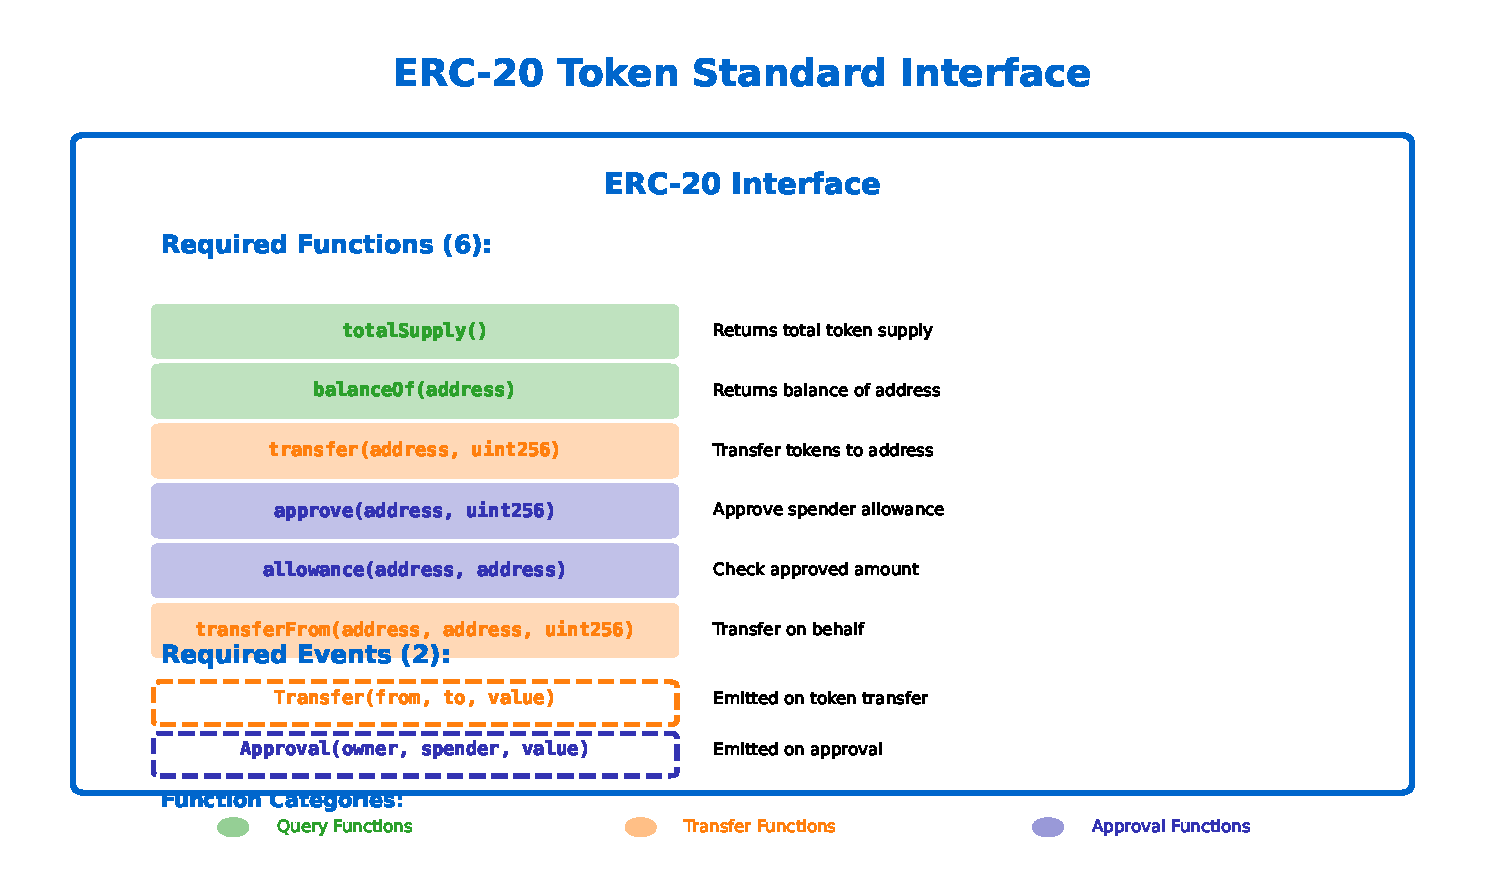
\includegraphics[width=0.85\textwidth]{01_erc20_interface/01_erc20_interface.pdf}
\end{center}

\bottomnote{Chart: Complete ERC-20 interface showing all 6 functions and 2 events with their signatures}
\end{frame}

% ==================== SLIDE 7: OTHER STANDARDS ====================
\begin{frame}[t]{Other Token Standards}
\begin{columns}[T]
\column{0.31\textwidth}
\textbf{ERC-721 (NFTs)}

Non-Fungible Tokens:
\begin{itemize}
\item Each token is unique
\item Has a \texttt{tokenId}
\item Digital collectibles
\item Art, gaming items
\item Proof of ownership
\end{itemize}

\vspace{0.3em}
\textit{Example:} CryptoPunks, Bored Apes

\column{0.31\textwidth}
\textbf{ERC-1155 (Multi-Token)}

Best of both worlds:
\begin{itemize}
\item Fungible AND non-fungible
\item Batch transfers
\item Gas efficient
\item Gaming use cases
\item Mixed collections
\end{itemize}

\vspace{0.3em}
\textit{Example:} OpenSea collections

\column{0.31\textwidth}
\textbf{ERC-4626 (Vaults)}

Tokenized yield vaults:
\begin{itemize}
\item Standardized yield
\item DeFi composability
\item Deposit/withdraw
\item Share accounting
\item Yield strategies
\end{itemize}

\vspace{0.3em}
\textit{Example:} Yearn vaults
\end{columns}

\vspace{0.5em}
\begin{center}
\begin{tabular}{lccc}
\toprule
\textbf{Standard} & \textbf{Fungible} & \textbf{Use Case} & \textbf{Year} \\
\midrule
ERC-20 & Yes & Currencies, utility & 2015 \\
ERC-721 & No & Collectibles, art & 2018 \\
ERC-1155 & Both & Gaming, mixed & 2019 \\
\bottomrule
\end{tabular}
\end{center}

\bottomnote{This lesson focuses on ERC-20; ERC-721 and ERC-1155 require additional complexity}
\end{frame}

% ==================== SECTION 2: ERC-20 FUNCTIONS ====================
\section{ERC-20 Functions Deep Dive}

\begin{frame}[t]
\vfill
\centering
\begin{beamercolorbox}[sep=8pt,center]{title}
\usebeamerfont{title}\Large Section 2: ERC-20 Functions Deep Dive\par
\end{beamercolorbox}
\begin{center}
\textit{Understanding each function in detail}
\end{center}
\vfill
\end{frame}

% ==================== SLIDE 8: TOTALSUPPLY AND BALANCEOF ====================
\begin{frame}[t,fragile]{Read Functions: totalSupply() and balanceOf()}
\begin{columns}[T]
\column{0.48\textwidth}
\textbf{totalSupply()}

\begin{lstlisting}[style=solidity]
function totalSupply()
    external view returns (uint256);
\end{lstlisting}

\vspace{0.3em}
\begin{itemize}
\item Returns total tokens in existence
\item \texttt{view} --- reads state, no gas cost
\item Used by wallets and explorers
\item Can be fixed or dynamic
\end{itemize}

\vspace{0.3em}
\textbf{Example:}
\begin{itemize}
\item USDC: $\sim$25 billion tokens
\item Our token: 1,000,000 max
\end{itemize}

\column{0.48\textwidth}
\textbf{balanceOf(address)}

\begin{lstlisting}[style=solidity]
function balanceOf(address account)
    external view returns (uint256);
\end{lstlisting}

\vspace{0.3em}
\begin{itemize}
\item Returns balance of specific address
\item \texttt{view} --- no gas for external calls
\item Most frequently called function
\item Wallets use this constantly
\end{itemize}

\vspace{0.3em}
\textbf{Internal Storage:}
\begin{lstlisting}[style=solidity]
mapping(address => uint256)
    private _balances;
\end{lstlisting}
\end{columns}

\bottomnote{These are view functions --- they read blockchain state without modifying it (no transaction needed)}
\end{frame}

% ==================== SLIDE 9: TRANSFER ====================
\begin{frame}[t,fragile]{Direct Transfer: transfer()}
\begin{columns}[T]
\column{0.48\textwidth}
\textbf{Function Signature}

\begin{lstlisting}[style=solidity]
function transfer(
    address to,
    uint256 amount
) external returns (bool);
\end{lstlisting}

\vspace{0.3em}
\textbf{How It Works:}
\begin{enumerate}
\item Caller initiates transfer
\item Contract checks balance
\item Subtracts from sender
\item Adds to recipient
\item Emits \texttt{Transfer} event
\item Returns \texttt{true} on success
\end{enumerate}

\column{0.48\textwidth}
\textbf{Token Flow Diagram}
\begin{center}
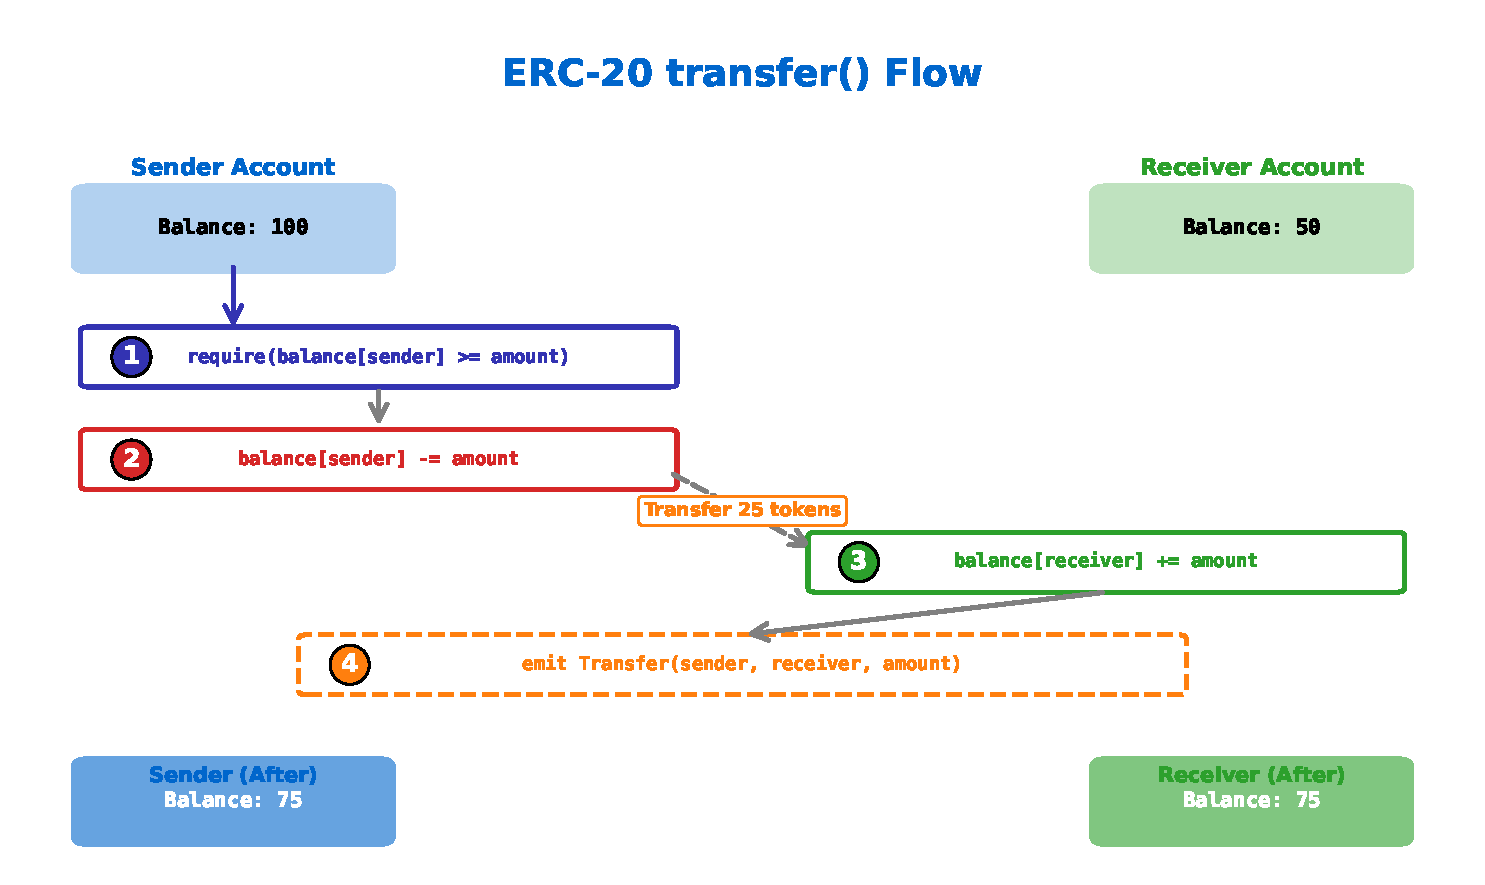
\includegraphics[width=\textwidth]{02_token_flow/02_token_flow.pdf}
\end{center}
\end{columns}

\vspace{0.3em}
\begin{lstlisting}[style=solidity]
// Internal implementation
function _transfer(address from, address to, uint256 amount) internal {
    require(from != address(0), "Transfer from zero address");
    require(to != address(0), "Transfer to zero address");
    require(_balances[from] >= amount, "Insufficient balance");
    _balances[from] -= amount;
    _balances[to] += amount;
    emit Transfer(from, to, amount);
}
\end{lstlisting}

\bottomnote{transfer() is for direct transfers from your wallet --- you control the tokens}
\end{frame}

% ==================== SLIDE 10: APPROVE AND ALLOWANCE ====================
\begin{frame}[t,fragile]{Delegation: approve() and allowance()}
\begin{columns}[T]
\column{0.48\textwidth}
\textbf{approve(spender, amount)}

\begin{lstlisting}[style=solidity]
function approve(
    address spender,
    uint256 amount
) external returns (bool);
\end{lstlisting}

\vspace{0.3em}
\textbf{Purpose:}
\begin{itemize}
\item Authorize another address to spend
\item Essential for DeFi interactions
\item Set spending limit (allowance)
\item Can be updated or revoked (set to 0)
\end{itemize}

\vspace{0.3em}
\begin{block}{Real-World Analogy}
\texttt{approve()} is like giving someone a \textbf{debit card with a spending limit}. You say ``you can spend up to \$1000 of my money.'' They can use it, but only up to that limit!
\end{block}

\column{0.48\textwidth}
\textbf{allowance(owner, spender)}

\begin{lstlisting}[style=solidity]
function allowance(
    address owner,
    address spender
) external view returns (uint256);
\end{lstlisting}

\vspace{0.3em}
\textbf{Purpose:}
\begin{itemize}
\item Check remaining allowance
\item Used before transferFrom
\item Wallets display this info
\item Returns 0 if none approved
\end{itemize}
\end{columns}

\vspace{0.3em}
\begin{center}
\textbf{Internal Storage:}
\begin{lstlisting}[style=solidity]
mapping(address => mapping(address => uint256)) private _allowances;
// _allowances[owner][spender] = amount
\end{lstlisting}
\end{center}

\bottomnote{Approvals enable smart contracts (DEXs, lending) to move tokens on your behalf}
\end{frame}

% ==================== SLIDE 11: TRANSFERFROM ====================
\begin{frame}[t,fragile]{Delegated Transfer: transferFrom()}
\begin{columns}[T]
\column{0.48\textwidth}
\textbf{Function Signature}

\begin{lstlisting}[style=solidity]
function transferFrom(
    address from,
    address to,
    uint256 amount
) external returns (bool);
\end{lstlisting}

\vspace{0.3em}
\textbf{How It Works:}
\begin{enumerate}
\item Spender calls transferFrom
\item Contract checks allowance
\item Contract checks balance
\item Deducts from allowance
\item Transfers tokens
\item Emits Transfer event
\end{enumerate}

\column{0.48\textwidth}
\textbf{Approval Flow}
\begin{center}
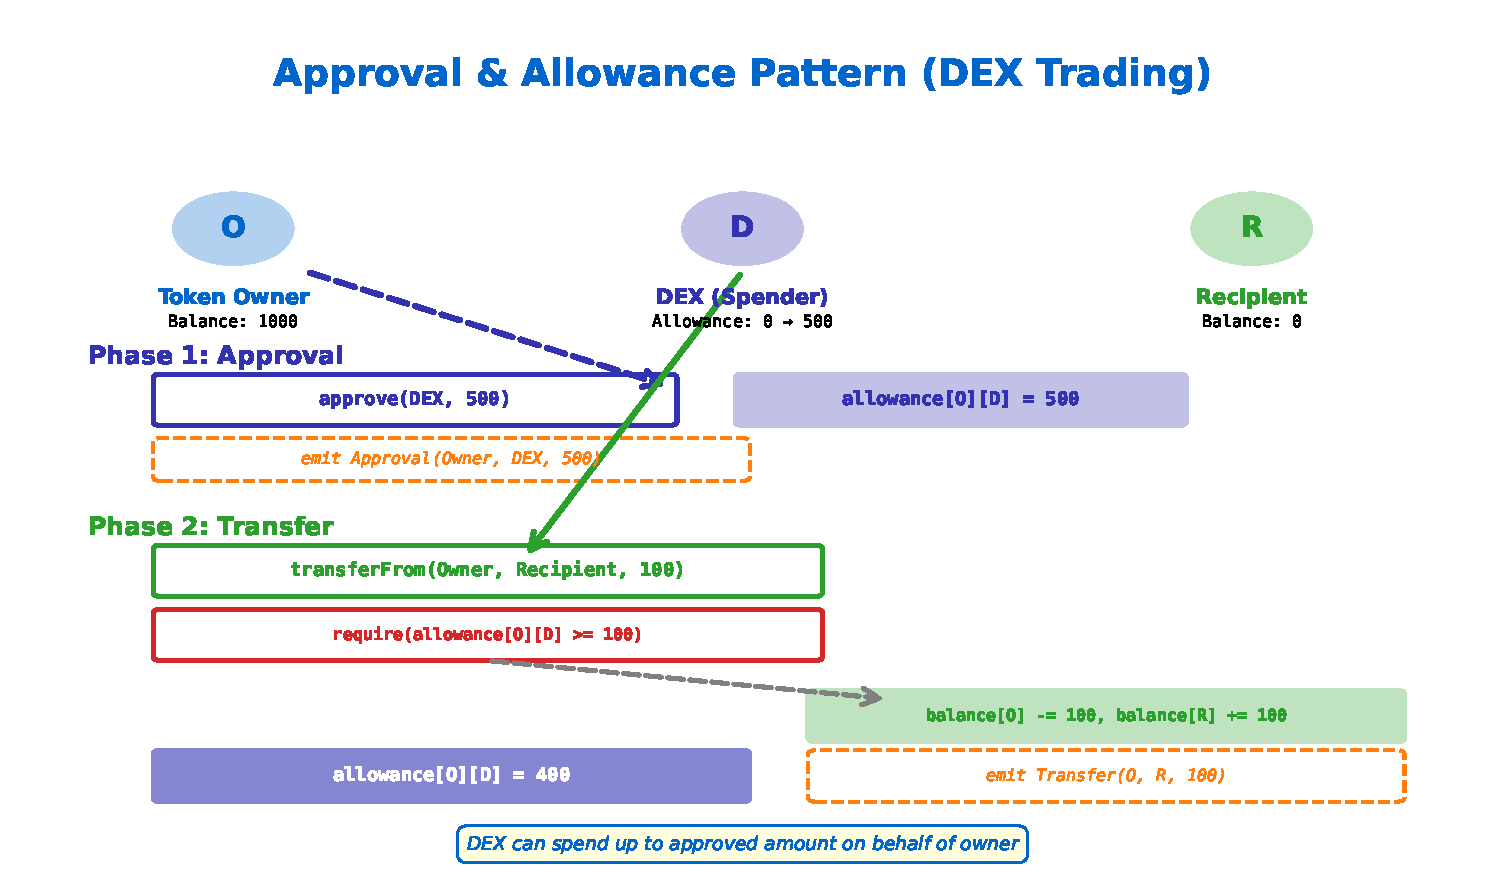
\includegraphics[width=\textwidth]{03_approval_allowance/03_approval_allowance.pdf}
\end{center}
\end{columns}

\vspace{0.3em}
\textbf{Real-World Example:}
\begin{enumerate}
\item You approve Uniswap to spend 1000 USDC
\item When you swap, Uniswap calls \texttt{transferFrom(you, pool, 500)}
\item Tokens move from your wallet to liquidity pool
\end{enumerate}

\bottomnote{transferFrom() is used by smart contracts --- requires prior approve() call}
\end{frame}

% ==================== SLIDE 12: EVENTS ====================
\begin{frame}[t,fragile]{Events: Transfer and Approval}
\begin{columns}[T]
\column{0.48\textwidth}
\textbf{Transfer Event}

\begin{lstlisting}[style=solidity]
event Transfer(
    address indexed from,
    address indexed to,
    uint256 value
);
\end{lstlisting}

\vspace{0.3em}
\textbf{Emitted When:}
\begin{itemize}
\item Tokens are transferred
\item Tokens are minted (from = 0x0)
\item Tokens are burned (to = 0x0)
\end{itemize}

\vspace{0.3em}
\textbf{Used By:}
\begin{itemize}
\item Block explorers (Etherscan)
\item Wallet notifications
\item DeFi dashboards
\end{itemize}

\column{0.48\textwidth}
\textbf{Approval Event}

\begin{lstlisting}[style=solidity]
event Approval(
    address indexed owner,
    address indexed spender,
    uint256 value
);
\end{lstlisting}

\vspace{0.3em}
\textbf{Emitted When:}
\begin{itemize}
\item Approval is granted
\item Approval is changed
\item Approval is revoked (value = 0)
\end{itemize}

\vspace{0.3em}
\textbf{Why \texttt{indexed}?}
\begin{itemize}
\item Enables efficient filtering
\item Can search by address
\item Max 3 indexed params
\end{itemize}
\end{columns}

\bottomnote{Events are stored in transaction logs --- cheap storage but cannot be read by contracts}
\end{frame}

% ==================== SLIDE 13: BASIC STRUCTURE ====================
\begin{frame}[t,fragile]{Code: Basic ERC-20 Structure}
\begin{lstlisting}[style=solidity]
// SPDX-License-Identifier: MIT
pragma solidity ^0.8.20;

contract BasicToken {
    string public name = "BasicToken";
    string public symbol = "BTK";
    uint8 public decimals = 18;
    uint256 public totalSupply;

    mapping(address => uint256) private _balances;
    mapping(address => mapping(address => uint256)) private _allowances;

    event Transfer(address indexed from, address indexed to, uint256 value);
    event Approval(address indexed owner, address indexed spender, uint256 value);

    constructor(uint256 initialSupply) {
        totalSupply = initialSupply * 10**decimals;
        _balances[msg.sender] = totalSupply;
        emit Transfer(address(0), msg.sender, totalSupply);
    }

    function balanceOf(address account) external view returns (uint256) {
        return _balances[account];
    }

    function transfer(address to, uint256 amount) external returns (bool) {
        require(_balances[msg.sender] >= amount, "Insufficient balance");
        _balances[msg.sender] -= amount;
        _balances[to] += amount;
        emit Transfer(msg.sender, to, amount);
        return true;
    }
    // ... approve, allowance, transferFrom
}
\end{lstlisting}

\bottomnote{This shows the minimal structure --- production code should use OpenZeppelin}
\end{frame}

% ==================== SLIDE 14: OPENZEPPELIN ====================
\begin{frame}[t,fragile]{Using OpenZeppelin}
\begin{columns}[T]
\column{0.48\textwidth}
\textbf{Why OpenZeppelin?}

\begin{itemize}
\item[\textcolor{mlgreen}{$\checkmark$}] Battle-tested code
\item[\textcolor{mlgreen}{$\checkmark$}] Security audited
\item[\textcolor{mlgreen}{$\checkmark$}] Industry standard
\item[\textcolor{mlgreen}{$\checkmark$}] Modular extensions
\item[\textcolor{mlgreen}{$\checkmark$}] Regular updates
\item[\textcolor{mlgreen}{$\checkmark$}] Community support
\end{itemize}

\vspace{0.3em}
\textbf{Installation:}
\begin{lstlisting}[style=javascript,numbers=none]
npm install @openzeppelin/contracts
\end{lstlisting}

\column{0.48\textwidth}
\textbf{Minimal ERC-20 Token}

\begin{lstlisting}[style=solidity]
// SPDX-License-Identifier: MIT
pragma solidity ^0.8.20;

import "@openzeppelin/contracts/
    token/ERC20/ERC20.sol";

contract SimpleToken is ERC20 {
    constructor()
        ERC20("SimpleToken", "STK")
    {
        _mint(msg.sender,
              1000000 * 10**decimals());
    }
}
\end{lstlisting}

\vspace{0.3em}
\textbf{That's it!} 8 lines for a complete, secure ERC-20 token.
\end{columns}

\bottomnote{OpenZeppelin is the gold standard for smart contract development --- never reinvent the wheel}
\end{frame}

% ==================== SECTION 3: BUILD MYTOKEN ====================
\section{Build MyToken}

\begin{frame}[t]
\vfill
\centering
\begin{beamercolorbox}[sep=8pt,center]{title}
\usebeamerfont{title}\Large Section 3: Build MyToken\par
\end{beamercolorbox}
\begin{center}
\textit{Hands-on: Creating a complete ERC-20 token}
\end{center}
\vfill
\end{frame}

% ==================== SLIDE 15: TOKEN SPECIFICATION ====================
\begin{frame}[t]{Our Token Specification}
\begin{columns}[T]
\column{0.48\textwidth}
\textbf{MyToken (MTK) Features}

\begin{tabular}{ll}
\toprule
\textbf{Property} & \textbf{Value} \\
\midrule
Name & MyToken \\
Symbol & MTK \\
Decimals & 18 \\
Max Supply & 1,000,000 MTK \\
Initial Supply & 100,000 MTK \\
\bottomrule
\end{tabular}

\vspace{0.5em}
\textbf{Custom Functions:}
\begin{itemize}
\item \texttt{mint()} --- Owner can create tokens
\item \texttt{burn()} --- Anyone can destroy tokens
\item \texttt{burnFrom()} --- Burn with allowance
\item \texttt{batchTransfer()} --- Multiple transfers
\end{itemize}

\column{0.48\textwidth}
\textbf{Inherited Features}

From \textbf{ERC20.sol}:
\begin{itemize}
\item All 6 standard functions
\item Both standard events
\item Decimal handling
\item Safe math (Solidity 0.8+)
\end{itemize}

\vspace{0.3em}
From \textbf{Ownable.sol}:
\begin{itemize}
\item Owner management
\item \texttt{onlyOwner} modifier
\item Ownership transfer
\item Renounce ownership
\end{itemize}

\vspace{0.3em}
\textbf{Design Decision:}\\
Max supply cap prevents unlimited inflation.
\end{columns}

\bottomnote{This design balances simplicity with useful features for learning and experimentation}
\end{frame}

% ==================== SLIDE 16: IMPORTS ====================
\begin{frame}[t,fragile]{Code: MyToken.sol Imports and Setup}
\begin{lstlisting}[style=solidity]
// SPDX-License-Identifier: MIT
pragma solidity ^0.8.20;

import "@openzeppelin/contracts/token/ERC20/ERC20.sol";
import "@openzeppelin/contracts/access/Ownable.sol";

/**
 * @title MyToken
 * @dev ERC-20 token implementation with minting and burning capabilities
 * @notice This contract demonstrates standard token functionality
 */
contract MyToken is ERC20, Ownable {
    // Maximum supply cap for the token
    uint256 public constant MAX_SUPPLY = 1000000 * 10**18;  // 1 million tokens

    // Contract body follows...
}
\end{lstlisting}

\vspace{0.3em}
\begin{columns}[T]
\column{0.48\textwidth}
\textbf{Key Elements:}
\begin{itemize}
\item SPDX license identifier (required)
\item Solidity version pragma
\item OpenZeppelin imports
\item NatSpec documentation
\end{itemize}

\column{0.48\textwidth}
\textbf{Inheritance:}
\begin{itemize}
\item \texttt{is ERC20} --- Token functions
\item \texttt{is Ownable} --- Access control
\item Multiple inheritance with comma
\item Order matters for constructors
\end{itemize}
\end{columns}

\bottomnote{The constant MAX\_SUPPLY is stored in contract bytecode, not storage (gas efficient)}
\end{frame}

% ==================== SLIDE 17: CONSTRUCTOR ====================
\begin{frame}[t,fragile]{Code: Constructor and Initial Minting}
\begin{lstlisting}[style=solidity]
/**
 * @dev Constructor that initializes the token
 * @notice Mints initial supply to the contract deployer
 */
constructor() ERC20("MyToken", "MTK") Ownable(msg.sender) {
    // Mint 100,000 tokens to the deployer (10% of max supply)
    _mint(msg.sender, 100000 * 10**18);
}
\end{lstlisting}

\vspace{0.5em}
\begin{columns}[T]
\column{0.48\textwidth}
\textbf{Constructor Breakdown:}
\begin{enumerate}
\item \texttt{ERC20("MyToken", "MTK")}
\begin{itemize}
\item Sets token name
\item Sets token symbol
\end{itemize}
\item \texttt{Ownable(msg.sender)}
\begin{itemize}
\item Sets deployer as owner
\item Enables access control
\end{itemize}
\item \texttt{\_mint(msg.sender, ...)}
\begin{itemize}
\item Creates initial tokens
\item Assigns to deployer
\end{itemize}
\end{enumerate}

\column{0.48\textwidth}
\textbf{Why \texttt{10**18}?}

ERC-20 tokens use 18 decimals by default:
\begin{itemize}
\item 1 token = $10^{18}$ base units
\item Like 1 ETH = $10^{18}$ wei
\item Enables fractional amounts
\item \texttt{100000 * 10**18} = 100,000 tokens
\end{itemize}

\vspace{0.3em}
\textbf{Initial Distribution:}\\
10\% to deployer, 90\% available for minting
\end{columns}

\bottomnote{The \_mint function is internal --- it creates tokens ``from nothing'' (from address 0)}
\end{frame}

% ==================== SLIDE 18: CUSTOM FEATURES ====================
\begin{frame}[t,fragile]{Code: Custom Features (Mint and Burn)}
\begin{lstlisting}[style=solidity]
/**
 * @dev Mint new tokens to a specified address
 * @param to Address that will receive the minted tokens
 * @param amount Amount of tokens to mint (in wei)
 */
function mint(address to, uint256 amount) public onlyOwner {
    require(to != address(0), "Cannot mint to zero address");
    require(totalSupply() + amount <= MAX_SUPPLY, "Exceeds max supply");
    _mint(to, amount);
}

/**
 * @dev Burn tokens from the caller's balance
 * @param amount Amount of tokens to burn
 */
function burn(uint256 amount) public {
    _burn(msg.sender, amount);
}

/**
 * @dev Burn tokens from a specified address (requires allowance)
 */
function burnFrom(address from, uint256 amount) public {
    _spendAllowance(from, msg.sender, amount);
    _burn(from, amount);
}
\end{lstlisting}

\bottomnote{mint() has supply cap protection | burn() is deflationary | burnFrom() requires approval}
\end{frame}

% ==================== SLIDE 19: FULL CONTRACT ====================
\begin{frame}[t,fragile]{Code: Full Contract Walkthrough}
\begin{columns}[T]
\column{0.48\textwidth}
\textbf{Contract Structure}

\begin{lstlisting}[style=solidity,numbers=none]
contract MyToken is ERC20, Ownable {
    // 1. State Variables
    uint256 public constant MAX_SUPPLY;

    // 2. Constructor
    constructor() { ... }

    // 3. Core Functions
    function mint() onlyOwner { ... }
    function burn() public { ... }
    function burnFrom() public { ... }

    // 4. View Functions
    function decimals() override { ... }

    // 5. Utility Functions
    function batchTransfer() public { ... }
}
\end{lstlisting}

\column{0.48\textwidth}
\textbf{Batch Transfer Feature}

\begin{lstlisting}[style=solidity]
function batchTransfer(
    address[] calldata recipients,
    uint256[] calldata amounts
) public {
    require(
        recipients.length == amounts.length,
        "Arrays length mismatch"
    );
    for (uint256 i = 0;
         i < recipients.length; i++) {
        _transfer(
            msg.sender,
            recipients[i],
            amounts[i]
        );
    }
}
\end{lstlisting}

\textbf{Use Case:} Airdrops, payroll
\end{columns}

\bottomnote{Full source: code/MyToken.sol | Total: 82 lines including documentation}
\end{frame}

% ==================== SLIDE 20: COMPILE ====================
\begin{frame}[t,fragile]{Compile with Hardhat}
\begin{columns}[T]
\column{0.48\textwidth}
\textbf{Project Setup}

\begin{lstlisting}[style=javascript,numbers=none]
# Initialize project
mkdir my-token && cd my-token
npm init -y
npm install --save-dev hardhat
npx hardhat init

# Install OpenZeppelin
npm install @openzeppelin/contracts
\end{lstlisting}

\vspace{0.3em}
\textbf{Project Structure:}
\begin{lstlisting}[style=javascript,numbers=none]
my-token/
  contracts/
    MyToken.sol
  scripts/
    deploy.js
  test/
    MyToken.test.js
  hardhat.config.js
  package.json
\end{lstlisting}

\column{0.48\textwidth}
\textbf{Compilation}

\begin{lstlisting}[style=javascript,numbers=none]
# Compile contracts
npx hardhat compile

# Expected output:
Compiling 1 file with 0.8.20
Compilation finished successfully
\end{lstlisting}

\vspace{0.3em}
\textbf{Compilation Artifacts:}
\begin{itemize}
\item \texttt{artifacts/} --- ABI and bytecode
\item \texttt{cache/} --- Build cache
\item ABI used for frontend integration
\item Bytecode deployed to blockchain
\end{itemize}

\vspace{0.3em}
\textbf{Common Errors:}
\begin{itemize}
\item Version mismatch in pragma
\item Missing OpenZeppelin install
\item Syntax errors in Solidity
\end{itemize}
\end{columns}

\bottomnote{Hardhat is the most popular Ethereum development environment --- alternatives: Foundry, Truffle}
\end{frame}

% ==================== SLIDE 21: DEPLOY SCRIPT ====================
\begin{frame}[t,fragile]{Deploy Script}
\begin{lstlisting}[style=javascript]
// scripts/deploy.js - Hardhat deployment script
const hre = require("hardhat");

async function main() {
  console.log("Starting MyToken deployment...\n");

  // Get the contract factory
  const MyToken = await hre.ethers.getContractFactory("MyToken");

  // Get deployer account
  const [deployer] = await hre.ethers.getSigners();
  console.log("Deploying with account:", deployer.address);

  // Deploy the contract
  const token = await MyToken.deploy();
  await token.waitForDeployment();

  const tokenAddress = await token.getAddress();
  console.log("MyToken deployed to:", tokenAddress);

  // Verify deployment
  const name = await token.name();
  const symbol = await token.symbol();
  const totalSupply = await token.totalSupply();
  console.log(`Token: ${name} (${symbol})`);
  console.log(`Total Supply: ${hre.ethers.formatUnits(totalSupply, 18)}`);
}

main().catch((error) => { console.error(error); process.exit(1); });
\end{lstlisting}

\bottomnote{Run with: npx hardhat run scripts/deploy.js --network localhost}
\end{frame}

% ==================== SLIDE 22: TESTING ====================
\begin{frame}[t,fragile]{Testing the Token}
\begin{columns}[T]
\column{0.48\textwidth}
\textbf{Local Testing Steps}

\begin{enumerate}
\item Start local blockchain:
\begin{lstlisting}[style=javascript,numbers=none]
npx hardhat node
\end{lstlisting}

\item Deploy to local network:
\begin{lstlisting}[style=javascript,numbers=none]
npx hardhat run scripts/deploy.js
  --network localhost
\end{lstlisting}

\item Run test suite:
\begin{lstlisting}[style=javascript,numbers=none]
npx hardhat test
\end{lstlisting}
\end{enumerate}

\vspace{0.3em}
\textbf{Hardhat Console:}
\begin{lstlisting}[style=javascript,numbers=none]
npx hardhat console --network localhost
> const Token = await ethers.
    getContractFactory("MyToken")
> const token = await Token.attach(
    "0x5FbDB...")
> await token.balanceOf(deployer)
\end{lstlisting}

\column{0.48\textwidth}
\textbf{Sample Test Cases}

\begin{lstlisting}[style=javascript]
describe("MyToken", function() {
  it("Should have correct name",
    async function() {
      expect(await token.name())
        .to.equal("MyToken");
  });

  it("Should mint initial supply",
    async function() {
      const balance = await token
        .balanceOf(owner.address);
      expect(balance).to.equal(
        ethers.parseEther("100000")
      );
  });

  it("Should transfer tokens",
    async function() {
      await token.transfer(
        addr1.address,
        ethers.parseEther("100")
      );
      // ... assertions
  });
});
\end{lstlisting}
\end{columns}

\bottomnote{Always test thoroughly on local network before deploying to testnet or mainnet}
\end{frame}

% ==================== SECTION 4: TOKEN ECONOMICS ====================
\section{Token Economics}

\begin{frame}[t]
\vfill
\centering
\begin{beamercolorbox}[sep=8pt,center]{title}
\usebeamerfont{title}\Large Section 4: Token Economics\par
\end{beamercolorbox}
\begin{center}
\textit{Designing sustainable token models}
\end{center}
\vfill
\end{frame}

% ==================== SLIDE 23: SUPPLY MODELS CHART ====================
\begin{frame}[t]{Token Supply Models}
\begin{center}
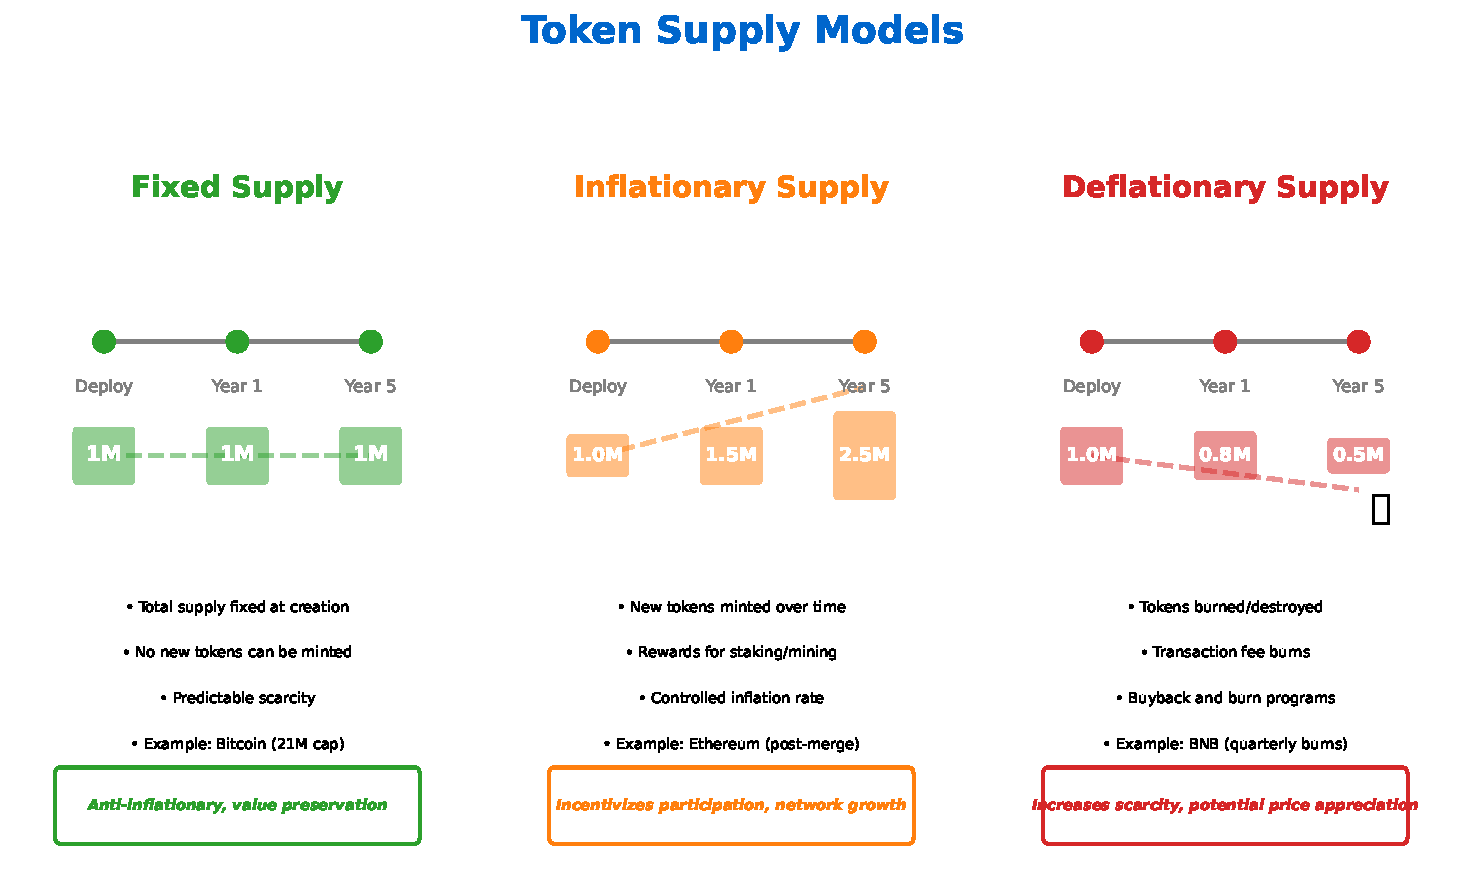
\includegraphics[width=0.85\textwidth]{05_token_economics/05_token_economics.pdf}
\end{center}

\bottomnote{Chart: Comparison of fixed, inflationary, and deflationary supply models over time}
\end{frame}

% ==================== SLIDE 24: SUPPLY COMPARISON ====================
\begin{frame}[t,fragile]{Fixed vs Inflationary vs Deflationary}
\begin{columns}[T]
\column{0.31\textwidth}
\textbf{Fixed Supply}

\textit{``Digital Gold''}
\begin{itemize}
\item Supply set at creation
\item Cannot mint more
\item Scarcity drives value
\item Example: Bitcoin (21M)
\end{itemize}

\vspace{0.3em}
\textbf{Code:}
\begin{lstlisting}[style=solidity,numbers=none]
constructor() {
  _mint(msg.sender,
        MAX_SUPPLY);
  // No mint function
}
\end{lstlisting}

\column{0.31\textwidth}
\textbf{Inflationary}

\textit{``Rewards \& Growth''}
\begin{itemize}
\item New tokens created
\item Rewards for staking
\item Funds development
\item Example: ETH (post-merge)
\end{itemize}

\vspace{0.3em}
\textbf{Code:}
\begin{lstlisting}[style=solidity,numbers=none]
function mint(
  address to,
  uint256 amount
) public onlyOwner {
  _mint(to, amount);
}
\end{lstlisting}

\column{0.31\textwidth}
\textbf{Deflationary}

\textit{``Burn to Earn''}
\begin{itemize}
\item Tokens destroyed
\item Fee burns
\item Increasing scarcity
\item Example: BNB
\end{itemize}

\vspace{0.3em}
\textbf{Code:}
\begin{lstlisting}[style=solidity,numbers=none]
function transfer(...) {
  uint256 fee = amount/100;
  _burn(from, fee);
  _transfer(from, to,
            amount - fee);
}
\end{lstlisting}
\end{columns}

\vspace{0.3em}
\begin{center}
\textbf{Our Token (MTK):} Hybrid --- Capped inflation with optional burning
\end{center}

\bottomnote{Token economics (tokenomics) significantly impacts long-term value and utility}
\end{frame}

% ==================== SLIDE 25: DISTRIBUTION ====================
\begin{frame}[t]{Distribution Strategies}
\begin{columns}[T]
\column{0.48\textwidth}
\textbf{Common Distribution Methods}

\begin{tabular}{lc}
\toprule
\textbf{Method} & \textbf{Typical \%} \\
\midrule
Team \& Founders & 15-20\% \\
Investors/VCs & 10-20\% \\
Public Sale (ICO/IDO) & 10-30\% \\
Community/Airdrops & 10-20\% \\
Ecosystem Fund & 20-30\% \\
Liquidity & 5-15\% \\
\bottomrule
\end{tabular}

\vspace{0.5em}
\textbf{Vesting Schedules:}
\begin{itemize}
\item Team tokens locked 1-4 years
\item Cliff period (6-12 months)
\item Linear or milestone unlocks
\item Prevents dump risk
\end{itemize}

\column{0.48\textwidth}
\textbf{Distribution Considerations}

\begin{itemize}
\item[\textcolor{mlgreen}{$\checkmark$}] \textbf{Fair Launch:} No pre-mine, equal access
\item[\textcolor{mlgreen}{$\checkmark$}] \textbf{Decentralization:} Avoid concentration
\item[\textcolor{mlgreen}{$\checkmark$}] \textbf{Incentive Alignment:} Team locked
\item[\textcolor{mlgreen}{$\checkmark$}] \textbf{Liquidity:} Tradeable from day 1
\end{itemize}

\vspace{0.5em}
\textbf{Red Flags:}
\begin{itemize}
\item[\textcolor{mlred}{$\times$}] Team holds >50\%
\item[\textcolor{mlred}{$\times$}] No vesting schedule
\item[\textcolor{mlred}{$\times$}] Hidden wallets
\item[\textcolor{mlred}{$\times$}] Unlimited minting
\end{itemize}
\end{columns}

\bottomnote{Transparent tokenomics build trust --- always publish distribution details}
\end{frame}

% ==================== SLIDE 26: REAL EXAMPLES ====================
\begin{frame}[t]{Real-World Token Examples}
\begin{center}
\begin{tabular}{lcccc}
\toprule
\textbf{Token} & \textbf{Type} & \textbf{Supply Model} & \textbf{Max Supply} & \textbf{Use Case} \\
\midrule
USDC & Stablecoin & Elastic & Unlimited & Payments \\
LINK & Utility & Fixed & 1B & Oracle services \\
UNI & Governance & Inflationary & 1B + 2\%/yr & DEX voting \\
AAVE & Governance & Fixed & 16M & Lending protocol \\
BNB & Utility & Deflationary & 200M (burns) & Exchange fees \\
MATIC & Utility & Fixed & 10B & L2 scaling \\
\bottomrule
\end{tabular}
\end{center}

\vspace{0.5em}
\begin{columns}[T]
\column{0.48\textwidth}
\textbf{Successful Patterns:}
\begin{itemize}
\item Clear utility (not just speculation)
\item Sustainable tokenomics
\item Active development
\item Strong community
\end{itemize}

\column{0.48\textwidth}
\textbf{Questions to Ask:}
\begin{itemize}
\item Why does this need a token?
\item What creates demand?
\item Who controls supply?
\item What's the unlock schedule?
\end{itemize}
\end{columns}

\bottomnote{Study successful tokens to understand what makes sustainable token economics}
\end{frame}

% ==================== SLIDE 27: DEPLOYMENT WORKFLOW ====================
\begin{frame}[t]{Deployment Workflow}
\begin{center}
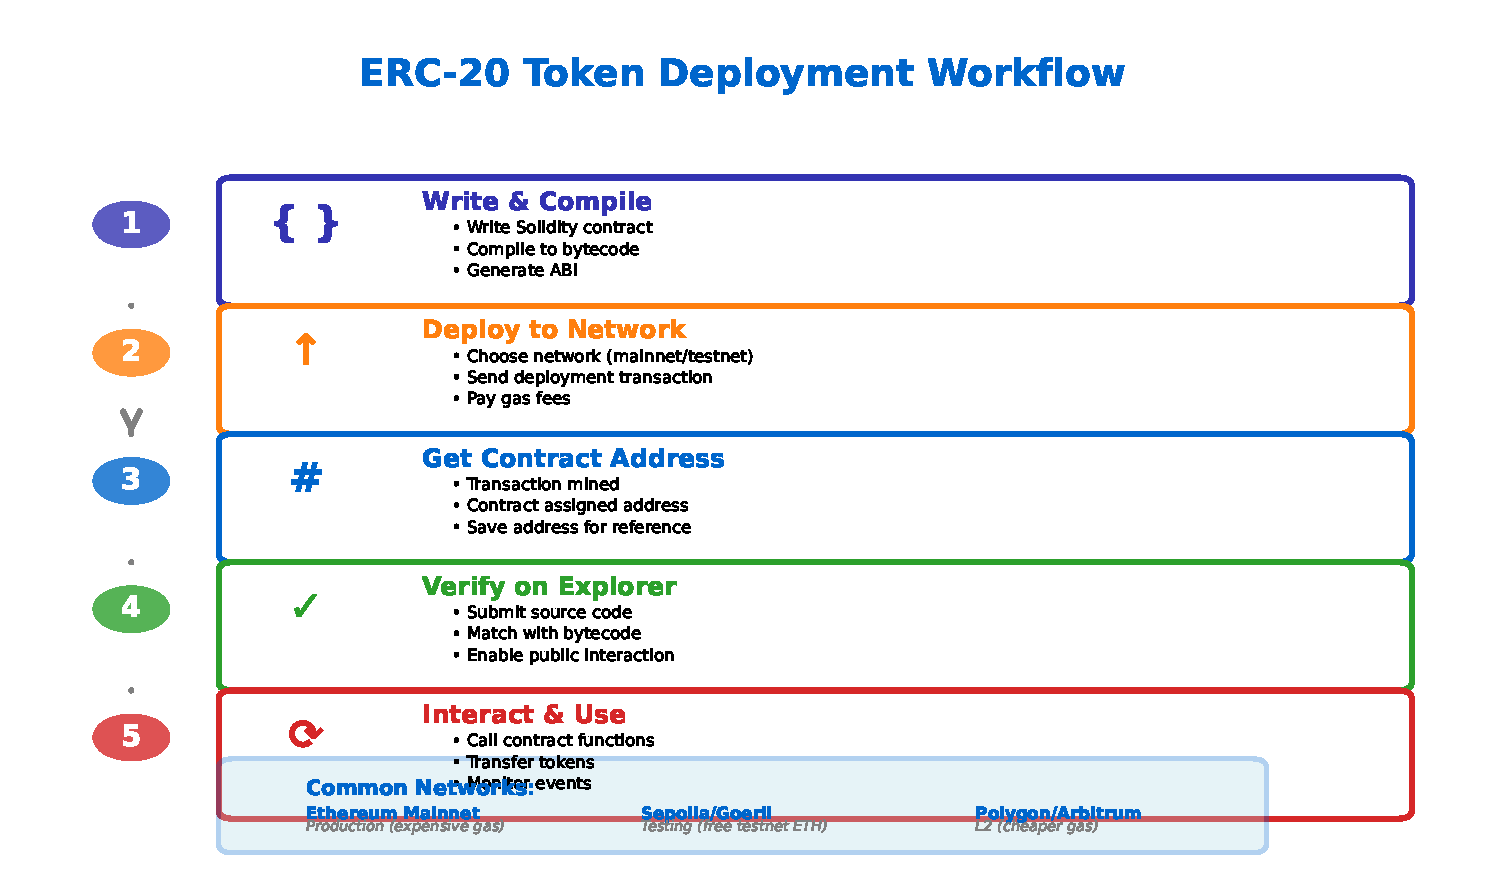
\includegraphics[width=0.9\textwidth]{04_deployment_steps/04_deployment_steps.pdf}
\end{center}

\bottomnote{Chart: Complete deployment workflow from development to mainnet launch}
\end{frame}

% ==================== SECTION 5: ADVANCED & SUMMARY ====================
\section{Advanced Topics \& Summary}

\begin{frame}[t]
\vfill
\centering
\begin{beamercolorbox}[sep=8pt,center]{title}
\usebeamerfont{title}\Large Section 5: Advanced Topics \& Summary\par
\end{beamercolorbox}
\begin{center}
\textit{Next steps and key takeaways}
\end{center}
\vfill
\end{frame}

% ==================== SLIDE 28: TESTNET DEPLOYMENT ====================
\begin{frame}[t,fragile]{Optional: Testnet Deployment}
\begin{columns}[T]
\column{0.48\textwidth}
\textbf{Testnet Options}

\begin{tabular}{lcc}
\toprule
\textbf{Network} & \textbf{Faucet} & \textbf{Speed} \\
\midrule
Sepolia & Yes & Fast \\
Goerli & Limited & Medium \\
Mumbai (Polygon) & Yes & Fast \\
\bottomrule
\end{tabular}

\vspace{0.5em}
\textbf{Hardhat Config:}
\begin{lstlisting}[style=javascript,numbers=none]
networks: {
  sepolia: {
    url: process.env.SEPOLIA_URL,
    accounts: [process.env.PRIVATE_KEY]
  }
}
\end{lstlisting}

\column{0.48\textwidth}
\textbf{Deployment Steps}

\begin{enumerate}
\item Get testnet ETH from faucet
\item Configure network in Hardhat
\item Set environment variables
\item Deploy:
\begin{lstlisting}[style=javascript,numbers=none]
npx hardhat run scripts/deploy.js
  --network sepolia
\end{lstlisting}
\item Verify on Etherscan:
\begin{lstlisting}[style=javascript,numbers=none]
npx hardhat verify
  --network sepolia
  CONTRACT_ADDRESS
\end{lstlisting}
\end{enumerate}

\textbf{Cost:} Free (testnet ETH has no value)
\end{columns}

\bottomnote{Testnet deployment is essential practice before mainnet --- treat it like production}
\end{frame}

% ==================== SLIDE 29: SECURITY WARNING ====================
\begin{frame}[t]{Security Considerations}
\begin{alertblock}{IMPORTANT DISCLAIMER}
The code in this lesson is for \textbf{educational purposes only}. Do NOT deploy to mainnet without professional security audits. Real money is at stake on mainnet!
\end{alertblock}

\vspace{0.3em}
\begin{columns}[T]
\column{0.48\textwidth}
\textbf{Common Vulnerabilities}

\begin{itemize}
\item[\textcolor{mlred}{!}] \textbf{Reentrancy:} Recursive calls
\item[\textcolor{mlred}{!}] \textbf{Integer overflow:} Pre-0.8.0
\item[\textcolor{mlred}{!}] \textbf{Access control:} Missing checks
\item[\textcolor{mlred}{!}] \textbf{Front-running:} MEV attacks
\item[\textcolor{mlred}{!}] \textbf{Approval race:} approve() issue
\end{itemize}

\vspace{0.3em}
\textbf{Before Mainnet:}
\begin{itemize}
\item Professional audit (\$5k-\$100k+)
\item Bug bounty program
\item Testnet battle-testing
\item Formal verification
\end{itemize}

\column{0.48\textwidth}
\textbf{Security Best Practices}

\begin{itemize}
\item[\textcolor{mlgreen}{$\checkmark$}] Use OpenZeppelin contracts
\item[\textcolor{mlgreen}{$\checkmark$}] Follow checks-effects-interactions
\item[\textcolor{mlgreen}{$\checkmark$}] Use \texttt{ReentrancyGuard}
\item[\textcolor{mlgreen}{$\checkmark$}] Implement \texttt{Pausable}
\item[\textcolor{mlgreen}{$\checkmark$}] Use multi-sig for ownership
\item[\textcolor{mlgreen}{$\checkmark$}] Test edge cases extensively
\end{itemize}

\vspace{0.3em}
\textbf{Security Resources:}
\begin{itemize}
\item Slither (static analysis)
\item Mythril (symbolic execution)
\item OpenZeppelin Defender
\item Consensys Diligence
\end{itemize}
\end{columns}

\bottomnote{Smart contract bugs are permanent and can result in total loss of funds}
\end{frame}

% ==================== SLIDE 30: FINAL PROJECT ====================
\begin{frame}[t]{Final Project Overview}
\begin{columns}[T]
\column{0.48\textwidth}
\textbf{Project: Custom Token}

Create your own ERC-20 token with:
\begin{enumerate}
\item Custom name and symbol
\item Defined tokenomics (supply model)
\item At least one custom feature
\item Comprehensive test suite
\item Deployed to testnet
\end{enumerate}

\vspace{0.3em}
\textbf{Bonus Challenges:}
\begin{itemize}
\item Add token burning on transfer
\item Implement vesting schedule
\item Create airdrop function
\item Add permit (EIP-2612)
\end{itemize}

\column{0.48\textwidth}
\textbf{Deliverables}

\begin{itemize}
\item \texttt{MyToken.sol} --- Contract code
\item \texttt{deploy.js} --- Deployment script
\item \texttt{test/*.js} --- Test files
\item README with tokenomics
\item Testnet deployment address
\item Etherscan verification
\end{itemize}

\vspace{0.3em}
\textbf{Evaluation Criteria:}
\begin{itemize}
\item Code quality and documentation
\item Test coverage (>80\%)
\item Security considerations
\item Creative features
\item Working deployment
\end{itemize}
\end{columns}

\bottomnote{This project integrates all 4 lessons: blockchain, cryptography, smart contracts, and tokens}
\end{frame}

% ==================== SLIDE 31: KEY TAKEAWAYS ====================
\begin{frame}[t]{Key Takeaways}
\begin{columns}[T]
\column{0.48\textwidth}
\textbf{What We Learned}

\begin{enumerate}
\item \textbf{Token Standards}
\begin{itemize}
\item \checkmark ERC-20 defines fungible tokens
\item \checkmark Standards enable interoperability
\item \checkmark 6 functions + 2 events required
\end{itemize}

\item \textbf{Core Functions}
\begin{itemize}
\item \checkmark transfer() for direct sends
\item \checkmark approve()/transferFrom() for delegation
\item \checkmark Events for transparency
\end{itemize}

\item \textbf{Development}
\begin{itemize}
\item \checkmark Use OpenZeppelin for security
\item \checkmark Use Hardhat for tooling
\item \checkmark Test extensively before deploy
\end{itemize}
\end{enumerate}

\column{0.48\textwidth}
\textbf{Key Concepts}

\begin{itemize}
\item[\textcolor{mlgreen}{$\checkmark$}] Tokens are smart contracts
\item[\textcolor{mlgreen}{$\checkmark$}] Standards enable the ecosystem
\item[\textcolor{mlgreen}{$\checkmark$}] Inheritance simplifies code
\item[\textcolor{mlgreen}{$\checkmark$}] Tokenomics matter for success
\item[\textcolor{mlgreen}{$\checkmark$}] Security is paramount
\end{itemize}

\vspace{0.5em}
\textbf{Skills Acquired:}
\begin{itemize}
\item \checkmark Read and understand ERC-20
\item \checkmark Create custom tokens
\item \checkmark Deploy with Hardhat
\item \checkmark Design tokenomics
\item \checkmark Evaluate token projects
\end{itemize}
\end{columns}

\bottomnote{You now have the foundation to build, deploy, and evaluate ERC-20 tokens}
\end{frame}

% ==================== SLIDE 32: COURSE COMPLETION ====================
\begin{frame}[t]{Course Completion \& Next Steps}
\begin{columns}[T]
\column{0.48\textwidth}
\textbf{Course Summary}

\begin{tabular}{cl}
\toprule
\textbf{Lesson} & \textbf{Topic} \\
\midrule
1 & Blockchain Fundamentals \\
2 & Cryptography \& Security \\
3 & Ethereum \& Smart Contracts \\
4 & ERC-20 Token Creation \\
\bottomrule
\end{tabular}

\vspace{0.5em}
\textbf{You Can Now:}
\begin{itemize}
\item Understand blockchain architecture
\item Explain cryptographic security
\item Write Solidity smart contracts
\item Create and deploy tokens
\end{itemize}

\column{0.48\textwidth}
\textbf{Continue Learning}

\begin{itemize}
\item \textbf{NFTs:} ERC-721 \& ERC-1155
\item \textbf{DeFi:} AMMs, lending, yield
\item \textbf{DAOs:} Governance tokens
\item \textbf{L2 Scaling:} Rollups, sidechains
\item \textbf{Security:} Auditing, formal methods
\end{itemize}

\vspace{0.5em}
\textbf{Resources:}
\begin{itemize}
\item Ethereum.org documentation
\item OpenZeppelin Learn
\item CryptoZombies (interactive)
\item Alchemy University
\item Speedrun Ethereum
\end{itemize}
\end{columns}

\vspace{0.5em}
\begin{center}
\textbf{Congratulations on completing the course!}
\end{center}

\bottomnote{The blockchain space evolves rapidly --- continuous learning is essential}
\end{frame}

% ==================== CLOSING SLIDE ====================
\begin{frame}[plain]
\vspace{2cm}
\begin{center}
{\Large Thank You}\\[1cm]
{\normalsize Questions?}\\[2cm]
{\small \textbf{Course:} Create Your Own Cryptocurrency}\\[0.3cm]
{\small \textbf{Lesson 4:} ERC-20 Token Creation}\\[1cm]
\textcolor{mlgray}{\small Build. Deploy. Innovate.}
\end{center}
\end{frame}

\end{document}
